
All code was implemented in the Julia language due to the availability of \textit{packages} for subproblems of this work. In the next section, several components of the solution to the problem of optimization of impulsive maneuvers are detailed, along with its full formulation.

\section{Orbit Propagation}\label{sec:orbit_propagation}

The implementation of an orbit propagator concerns itself with the implementation of the function \(p_o(X, t)\) introduced in Equation~\eqref{eq:orbit_propagator}. Two different cases are to be considered: "explicit" propagation, where numerical inputs are available and a numerical output is desired; and "implicit" propagation, where the propagation step is a part of a larger solver.

Brazil's INPE developed a package for orbit propagation and analysis with several models (Kepler, J2 semi-analytical secular and short term, among others) called \texttt{SatelliteToolbox}. It provides quite convient functions for converting between the Cartesian state vector \(\begin{bmatrix}
    r^T & v^T
\end{bmatrix}^T\) and the Keplerian elements, as well as functions for the propagation of orbits by some specified amount of time \(t_p\). Its algorithms were chosen with precision around edge cases in mind~\cite{rv_to_kepler}, making it numerically precise but unsuitable for nonlinear solvers, which expect differentiable functions everywhere. The functions in this package are also limited to elliptic orbits.

Therefore, this is an auxiliary package used for verification, initial guess generation, and direct numerical propagation whenever required. When propagation is required in the statement of a nonlinear optimization problem, another method for orbit propagation is required. Discretized numerical integration in Cartesian coordinates was chosen for this. Discretized integration inside a numerical solver is done via collocation, direct shooting or multiple shooting (also known as relaxation). Multiple shooting was chosen since it leads to a sparse problem, which benefits the performance of the chosen solver (see next section)

Let \(X_{\text{next}} = f_{RK}(X_{\text{prev}}, \Delta t)\) be the (two-body) dynamics function discretized through a fourth order Runge Kutta method. Then a number \(N\) of integration steps is chosen and \(N+1\) state vector variables \(X^j, j=1,\dots,N+1\) are created beloning to an array \(\chi \in \mathbb{R}^{6 \times (N+1)}\). They are subject to the constraints
\begin{equation}
    X^{j+1} = f_{RK}(X^j, \frac{t_p}{N}), j = 1, \dots, N.
\end{equation}
This leaves \(\dim X = 6\) degrees of freedom, which are to be specified with a boundary condition. This boundary condition can be an initial condition, a final condition or relation to another coasting segment through an impulse, as will be discussed in Section~\ref{sec:impulsive_statement}. Thus, this parameterization of orbital propagation is \textit{isoconstrained}.

\section{Nonlinear solver}

Nonlinear solvers are algorithms which iteratively approximate the solution to a system of nonlinear equations or a constrained optimization problem. Many algorithms, and many different algorithms exist. Broadly speaking, there are two classes of algorithms: gradient-free and gradient based. Gradient-free methods do not rely on derivatives for finding a solution; prototypical examples are Simplex methods, evolutionary algorithms, and simulated annealing. They are quite general but do not fully exploit a problem's structure when derivative information is available. Gradient-based methods include gradient descent, sequential quadratic programming (SQP), Newton-Raphson, trust-region methods and interior point methods. A sophisticated implementation of an interior point method is found in Ipopt, an open-source solver with interfaces in many languages~\cite{ipopt}.

A further distinction between algorithms is whether they are local or global solvers. Local solvers will converge (usually quickly) to a local optimum, which is not certified to be the global optimum (and in general, should not be assumed to be). Thus they rely on good initial guesses, to be provided to the solver, to arrive at an extremum. Global solvers can discover multiple local extrema and select the best among them; they sometimes rely on multiple (possibly random) initial values for a local optimizer. Ipopt is a local solver.

Julia offers a multitude of nonlinear solvers, each with different scope, interface, and algorithms. This work has chosen to use \texttt{JuMP}, a package which offers a modelling language for optimization problems that is quite close to mathematical notation. The package's \textit{tech stack} can be seen in Figure~\ref{fig:tech_stack}. Internally, \texttt{JuMP} relies on an intermediary package, \texttt{MathOptInterface}, which standardizes solver interfaces. This in turn allows for the usage of \texttt{Ipopt\_jll}, an unofficial wrapper for the Ipopt solver. Ipopt is an open-source nonlinear solver widely recognized for its speed and precision, outperforming many competitors and being quite flexible. It is especially well suited to problems with many variables (up to thousands) with sparse constraints (that is, constraints that depend only on small subsets of variables). It is capable of handling equality and inequality constraints.

This solver allows for the specification of lower and upper bounds of variables separately to the specification of inequality constraints. Variable bounds are guaranteed to be respected at all iterations; inequality constraints are only guaranteed to be satisfied at the converged solution, if the problem is feasible. This distinction is important because some constraints define the domain of problem and should never be violated; other constraints are problem-based and therefore can be violated during the iteration process.

Finally, Ipopt is built with sparsity in mind. Complex calculations should be broken into simpler constraints, each depending on less variables. This may even increase the number of variables but Ipopt's performance profits from this structure.

\begin{figure}[htbp]
    \centering
        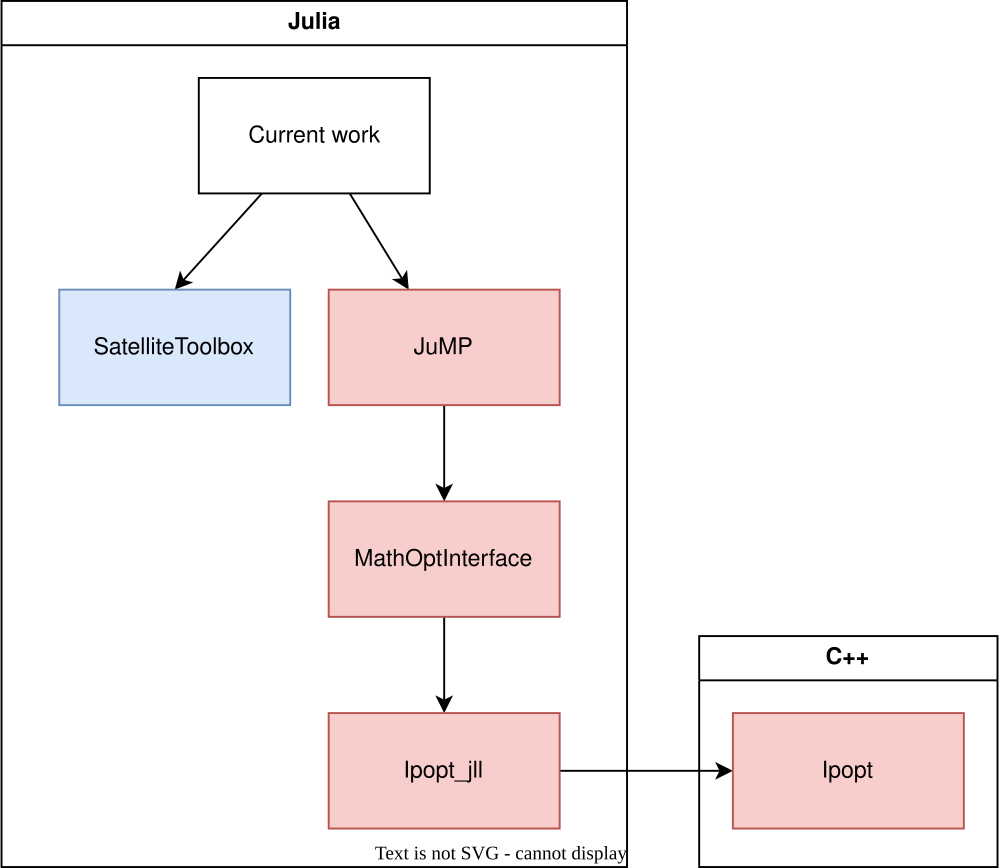
\includegraphics[width=\textwidth]{img/techstack.png}
    \caption{Relationship of code components}
    \label{fig:tech_stack}
\end{figure}

\section{Lambert problem implementation}

The formulations stated in the previous chapter make for one-dimensional nonlinear programs, which leads to high performance. However, they do not handle the singularity case of \(r_1 \parallel r_2\), which is of particular importance to orbital maneuvers as they often happen at periapsis and apoapsis. Sukhanov's formulation actually gives expressions for the initial radial and normal velocity when the input positions are collinear; the plane of the orbit should then be adequately chosen afterwards. However, this was found to be very numerically sensitive and another algorithm was used in the rest of this work. An implicit orbit propagation algorithm, as described in Section~\ref{sec:orbit_propagation} is setup with boundary conditions

\begin{align}
    r_{(j=1)} &= r_1 \\
    r_{(j=N+1)} &= r_2
\end{align}
which account for the 6 boundary conditions needed. In order to help convergence in the collinear case (and neighboring cases), two inequality constraints may be added:
\begin{align}
    r_j^T r_j &\geq R_{\text{Earth}}^2 \\
    r_j \times v_j &\geq 0
\end{align}
where the second constraint must be inverted if the desired orbit is retrograde. 

The propagation variables are initialized with the initial position and velocity.

\section{Optimal impulsive maneuver problem statement}\label{sec:impulsive_statement}

The full optimization problem, as it is implemented in code, shall be stated in this section. Due to \texttt{JuMP}'s intuitive modelling language, the problem is coded almost as it is stated here. The input parameters are:
\begin{enumerate}
    \item \(r_1\), \(v_1\): initial orbital position and velocity;
    \item \(r_2\), \(v_2\): final orbital position and velocity;
    \item \(t_f\): transfer time;
    \item \(N\): number of integration steps per coasting arc.
\end{enumerate}

The problem comprises the following variables, where inequalities represent variable bounds:
\begin{enumerate}
    \item \(\Delta t_1 \geq 0\), \(\Delta t_2 \geq 0\): intervals between 0 and the first maneuver and between the first and second maneuver;
    \item \(\Delta v_1 \geq 0\), \(\Delta v_2 \geq 0\)\footnote{The problem could have been parameterized with vector quantities for the changes in velocities, \(\Delta \vec v\), but the objective function would then be stated \(\sum \sqrt{\Delta \vec v^T \Delta \vec v}\), which is not differentiable at \(\Delta \vec v = 0\), which is inconvenient.}: magnitudes of the first and second impulses;
    \item \(\hat u 1\), \(\hat u_2 \in \mathbb{R}^3\): directions of the first and second impulses;
    \item \(\chi_1\), \(\chi_2\), \(\chi_3 \in \mathbb{R}^{6 \times (N+1)}\): arrays of state variables for each coasting arc. They shall be indexed as \(\chi_c^{kj}\), \(c=1, 2, 3\) is the coasting arc index, \(k=1,\dots,6\) is the component index, \(j = 1,\dots,N+1\) is the state vector index. \(X^j_c, r^j_c, v^j_c\) denote the j-th state , position and velocity vectors of the c-th coasting arc: \((X^j_c)_k = \chi_c^{kj}\).
\end{enumerate}

These variables are then subjected to constraints:
\begin{align}
    \text{Total time less than transfer time} &\qquad\Delta t_1 + \Delta t_2 \leq t_f \\
    \text{Unit directions} &\qquad\Delta \hat{u}_m^T \Delta \hat{u}_m = 1, m = 1, 2 \\
    \text{Initial state} &\qquad \chi_1^{k, 1} = \begin{bmatrix}
        r_1 \\ v_1
    \end{bmatrix}_k, k = 1,\dots, 6 \\
    \text{Final state} &\qquad \chi_3^{k, N+1} = \begin{bmatrix}
        r_2 \\ v_2
    \end{bmatrix}_k, k = 1,\dots, 6 \\
    \text{Maneuver boundary conditions} &\qquad \chi_{m+1}^{k, 1} = \chi_m^{k, N+1} + \begin{bmatrix}
        0_{3\times1} \\ \Delta v_m \hat{u}_m
    \end{bmatrix}, m=1, 2 \\
    \text{Propagation of coasting arcs} &\qquad X_c^{j+1} = f_{RK}(X_c^j, \Delta t_c / N), c=1, 2, 3, j=1,\dots,N \\
    \text{where} & \qquad \Delta t_3 = t_f - \Delta t_1 - \Delta t_2 \\
    % \text{Prograde orbit} &\qquad r^j_c \times v^j_c \geq 0, \forall j, c \\
    % \text{Non-intersection with Earth} &\qquad (r^j_c)^T r^j_c \geq R_{\text{Earth}}^2
\end{align}

Finally, the objective is given by
\begin{equation}
    \min \Delta v_1 + \Delta v_2
\end{equation}

The solver should be initialized with a feasible, but not necessarily optimal solution, for better convergence (since Ipopt is a local solver, the choice of initial guesses is important). Values for \(\Delta t_1\) and \(\Delta t_2\) should be proposed based on physical reasoning. Then, the variables of the first and last coasting arcs are initialized with direct orbital propagation results (computed with the \texttt{SatelliteToolbox} package). The second coasting arc, between the impulses, is initialized with the solution to the Lambert problem between the final position of the first coasting arc and the initial position of the last coasting arc. Finally, the variables concerning the impulses' magnitudes and directions are initialized with the difference in velocity between consecutive arcs.